\documentclass[tikz,border=10pt]{standalone}
\usetikzlibrary{shapes,arrows,positioning,calc,fit}

\begin{document}

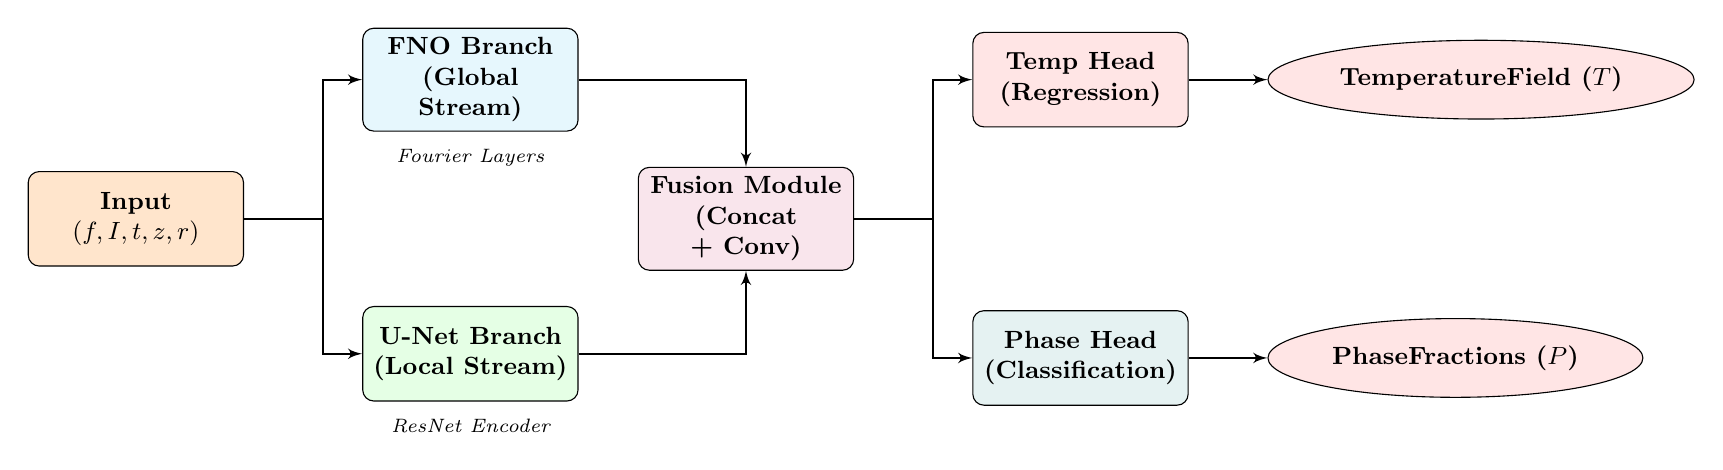
\begin{tikzpicture}[
    node distance=1.5cm,
    auto,
    block/.style={
        rectangle, 
        draw, 
        fill=blue!10, 
        text width=2.5cm, 
        text centered, 
        rounded corners, 
        minimum height=1.2cm,
        font=\small\bfseries
    },
    line/.style={
        draw, 
        -latex', 
        thick
    },
    cloud/.style={
        draw, 
        ellipse, 
        fill=red!10, 
        node distance=3cm,
        minimum height=1cm,
        font=\small\bfseries
    }
]

    % Nodes
    \node [block, fill=orange!20] (input) {Input\\$(f, I, t, z, r)$};
    
    % Split point
    \coordinate [right=1cm of input] (split);
    
    % Branches
    \node [block, fill=cyan!10, above right=0.5cm and 1.5cm of input] (fno) {FNO Branch\\(Global Stream)};
    \node [block, fill=green!10, below right=0.5cm and 1.5cm of input] (unet) {U-Net Branch\\(Local Stream)};
    
    % Fusion
    \node [block, fill=purple!10, right=4cm of split] (fusion) {Fusion Module\\(Concat + Conv)};
    
    % Heads
    \node [block, fill=red!10, above right=0.5cm and 1.5cm of fusion] (head_temp) {Temp Head\\(Regression)};
    \node [block, fill=teal!10, below right=0.5cm and 1.5cm of fusion] (head_phase) {Phase Head\\(Classification)};
    
    % Outputs
    \node [cloud, right=1cm of head_temp] (out_temp) {Temperature\\Field ($T$)};
    \node [cloud, right=1cm of head_phase] (out_phase) {Phase\\Fractions ($P$)};

    % Edges
    \path [line] (input) -- (split) |- (fno);
    \path [line] (input) -- (split) |- (unet);
    
    \path [line] (fno) -| (fusion);
    \path [line] (unet) -| (fusion);
    
    \coordinate [right=1cm of fusion] (split2);
    \path [line] (fusion) -- (split2) |- (head_temp);
    \path [line] (fusion) -- (split2) |- (head_phase);
    
    \path [line] (head_temp) -- (out_temp);
    \path [line] (head_phase) -- (out_phase);

    % Annotations
    \node [below=0.1cm of fno, font=\scriptsize\itshape] {Fourier Layers};
    \node [below=0.1cm of unet, font=\scriptsize\itshape] {ResNet Encoder};

\end{tikzpicture}

\end{document}
